%%%%%%%%%%%%%%%%%%%%%%%%%%%%%%%%%%%%%%%%%%%%%%%%%%%%%%%%%%%%%%%%%%%%%%%%%%%%%
%
%  System        : 
%  Module        : 
%  Object Name   : $RCSfile$
%  Revision      : $Revision$
%  Date          : $Date$
%  Author        : $Author$
%  Created By    : Robert Heller
%  Created       : Sat Mar 4 08:39:57 2023
%  Last Modified : <230307.1145>
%
%  Description 
%
%  Notes
%
%  History
% 
%%%%%%%%%%%%%%%%%%%%%%%%%%%%%%%%%%%%%%%%%%%%%%%%%%%%%%%%%%%%%%%%%%%%%%%%%%%%%
%
%    Copyright (C) 2023  Robert Heller D/B/A Deepwoods Software
%			51 Locke Hill Road
%			Wendell, MA 01379-9728
%
%    This program is free software; you can redistribute it and/or modify
%    it under the terms of the GNU General Public License as published by
%    the Free Software Foundation; either version 2 of the License, or
%    (at your option) any later version.
%
%    This program is distributed in the hope that it will be useful,
%    but WITHOUT ANY WARRANTY; without even the implied warranty of
%    MERCHANTABILITY or FITNESS FOR A PARTICULAR PURPOSE.  See the
%    GNU General Public License for more details.
%
%    You should have received a copy of the GNU General Public License
%    along with this program; if not, write to the Free Software
%    Foundation, Inc., 675 Mass Ave, Cambridge, MA 02139, USA.
%
% 
%
%%%%%%%%%%%%%%%%%%%%%%%%%%%%%%%%%%%%%%%%%%%%%%%%%%%%%%%%%%%%%%%%%%%%%%%%%%%%%

\documentclass[12pt,twoside]{article}
\usepackage{graphicx}
\usepackage{mathptm}
\usepackage{times}
\usepackage{makeidx}
\usepackage{ifpdf}
\usepackage{footmisc}
\ifpdf
\usepackage[pdftex,
            pagebackref=true,
            colorlinks=true,
            linkcolor=blue,
            unicode
           ]{hyperref}
\else
\usepackage[ps2pdf,
            pagebackref=true,
            colorlinks=true,
            linkcolor=blue,
            unicode
           ]{hyperref}
\usepackage{pspicture}
\fi
\usepackage{url}
\pagestyle{headings}
\makeindex
\emergencystretch=50pt
\setcounter{tocdepth}{3}
\setcounter{secnumdepth}{3}
\title{ESP32 T7S3 MultiFunctionUniversalTurnout Kit Instructions}
\author{Robert Heller \\ The Country Robot \\ Wendell, MA, USA}
\date{\today}
\begin{document}
\maketitle

This is a circuit board that supports a Lily Go T7 S3 (mini32) board to manage
multiple model railroad functions as a LCC\footnote{Layout Command Control --
see NMRA's 9.7.x standards, available on the NMRA website
\url{https://www.nmra.org/lcc}.} node. This board provides the following 
functions:

\begin{itemize}
\item Four turnout motors with point sense.  This board uses one of four 
turnout driver daughter boards:
\begin{enumerate}
\item Stall-motor drivers, suitable for Circuitron Tortoise and similar slow 
motion, stall motor switch machines.
\item Twin-coil drivers, suitable for Atlas or Peco snap action switch 
machines.
\item Single-coil drivers, suitable for Kato snap action switch machines.
\item Servo drivers, suitable for using RC control servos to operate turnouts.
\end{enumerate}
\item Four CT coil occupancy detectors.
\item Four driver circuits, suitable for indicator LEDs, decoupling 
electromagnets, solenoids, relays, etc.
\item Four Schmitt-trigger button inputs.
\item Sixteen signal lamp drivers.
\end{itemize}

\clearpage
\section{Assembly}
\begin{figure}[hbpt]\begin{centering}%
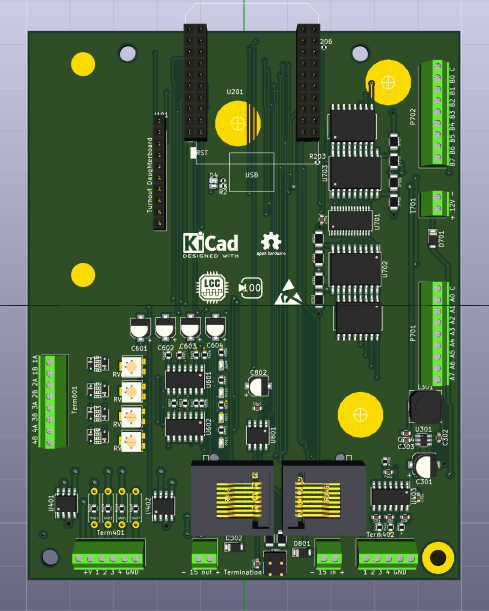
\includegraphics[width=4in]{ESP32-T7S3-MultiFunctionUniversalTurnout.png}
\caption{3D image of the ESP32 T7S3 MultiFunctionUniversalTurnout board}
\end{centering}\end{figure}
\begin{figure}[hbpt]\begin{centering}%
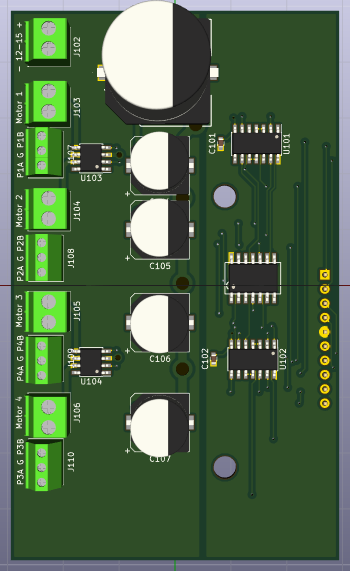
\includegraphics[height=3in]{SC-DaughterBoard.png}
\caption{3D image of the Single Coil Turnout driver daughter board}
\end{centering}\end{figure}
\begin{figure}[hbpt]\begin{centering}%
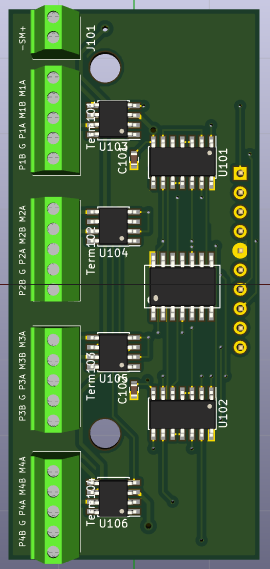
\includegraphics[height=3in]{SM-DaughterBoard.png}
\caption{3D image of the Stall Motor driver daughter board}
\end{centering}\end{figure}
\begin{figure}[hbpt]\begin{centering}%
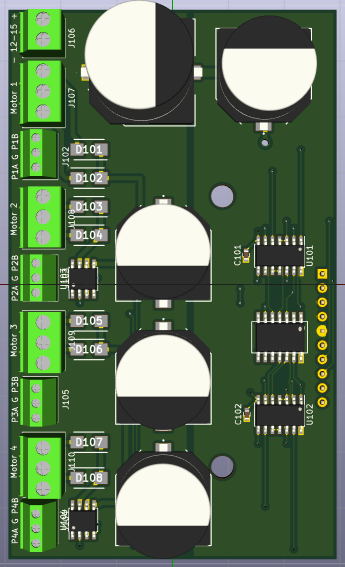
\includegraphics[height=3in]{TC-DaughterBoard.png}
\caption{3D image of the Twin Coil driver daughter board}
\end{centering}\end{figure}
\begin{figure}[hbpt]\begin{centering}%
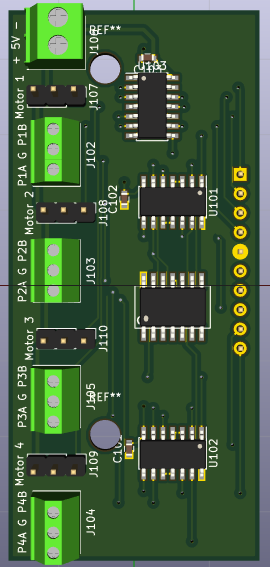
\includegraphics[height=3in]{TS-DaughterBoard.png}
\caption{3D image of the Servo driver daughter board}
\end{centering}\end{figure}
\clearpage

The boards have all of the SMD parts factory installed. Only the through-hole
parts are not soldered to the board. These are the RJ45 Jacks, the Termination
Jumper, the turnout daughter board header, the min32 headers, the daughter
board support standoffs, and the terminal blocks. The daughter boards also
have all of their SMD parts factory installed, and just needs their terminal
blocks and board inter-connect pin array headers installed. These are all easy
to solder parts. Make sure the headers and terminal blocks are fully seated
and square to the boards. A simple trick is to solder one pin and then while
pressing the part to the board, reheat that one pin's solder pad and snaping
the part to the board and holding it tight and square to the board as the
solder cools. Important: make sure the wire entry holes in the terminal blocks
are facing the edge of the board! The RJ45 Jacks cannot be installed wrong
(they have orientation pins). Start with the shortest parts and work up to the
tallest. Note: the pin array on the daughtboard goes on the bottom of the
board and is soldered on the top side.

%% Need photo of a daughter board's pin array.

\begin{figure}[hbpt]\begin{centering}%
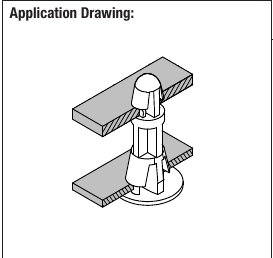
\includegraphics{NylonStandoffInstall.png}
\caption{Nylon Standoff Installation}
\end{centering}\end{figure}

The daughter boards are supported with a pair of nylon standoffs.  These are 
pushed through from the bottom of the main board.

You also need to solder the 2x10 pin headers to the bottom of the T7S3 board.

%% Add photo

Once all of the soldering is done, the T7S3 can be installed on the main board.
The WiFi antenna extends beyond the top of the board, with the T7S3's USB 
connector facing into the center of the board.  The daughter board's pin array 
goes in the socket header on the main board and there are two holes in the 
daughter board that engage the nylon standoffs.

%% Need a photo of a daughter board being installed on the main board 
%% and probably one of the T7S3 installed on the main board.

\clearpage
\section{Downloadables and Software Support}

As shipped, the TTGO-T7S3 has already had the ESP32-S3-MultiFunctionOpenMRNIDF
firmware installed, but if you want to rebuild the code (possibly with
customizations) the code is on GitHub in my ESP32-LCC repo:
\url{https://github.com/RobertPHeller/ESP32-LCC}, in the
ESP32-S3-MultiFunctionOpenMRNIDFOpenMRNIDF sub-folder. You will need the
Espressif's IoT Development Framework, version 4.2 or later, available from
\url{https://github.com/espressif/esp-idf}. The
ESP32-S3-MultiFunctionOpenMRNIDFOpenMRNIDF also uses Mike Dunston's OpenMRNIDF
module. Also available in the 
ESP32-T7S3-MultiFunctionUniversalTurnout/KitBooklet sub-folder are pdfs of the 
circuit diagrams.

\subsection{Building and installing the software}

Once you have installed Espressif's IoT Development Framework and cloned the 
ESP32-LCC repo, you can build the software by cd'ing to the 
ESP32-S3-MultiFunctionOpenMRNIDF and in bash running these commands:

\begin{verbatim}
. path-to-Espressifs-IDF/export.sh
idf.py set-target esp32s3
idf.py menuconfig
idf.py build
\end{verbatim}

Things to check in the menuconfig (under ``Advanced Configuration''):

\begin{itemize}
\item{Using TTGO-T7S3} Turn this option on.
\item{Using the servo turnout daughter board} If you are using the TS (turnout 
servo) daughter board, turn this on.  If using any of the other turnout 
daughter boards turn this off.
\end{itemize}

You can then use the idf.py's flash command to flash the TTGO-T7S3.

\subsection{Program Description}

The program consists of a main sketch file, and several support files and
``components'' (libraries).

\subsection{Program Startup notes}

While most of the common node configuration is accessable using the available
CDI configuruation tools (JMRI's PanelPro program or MRR SYS OpenLCB program),
some of the node's configuration is in separate non-volitle (flash) memory.
This includes the node's ID number and some boot options. As installed the
node ID is initialized to 05:01:01:01:22:00. \textbf{You don't really want to
leave this as the node id!} There are two ways to set the node id. One way is
to use a CDI configuruation tool -- the node ID is exposed as a configuration
option. Changing the node id forces a ``factory reset'' on the next boot (and
when you update the configuration with a CDI configuruation tool, the node
will reboot). The other way is during the boot up process. When the node
boots, it waits on the USB serial connection for 10 seconds for any
``keyboard'' response and if it gets a ``keyboard'' response, it enters a
simple command line loop accepting simple commands (mostly single letters). To
use this feature you need to connect a a USB cable between the TTGO-T7S3 and a
computer (eg a PC or Mac) and then connect to the USB Com port with a terminal
program (the Arduino IDE Serial Monitor should work). The commands that the
boot startup command line loop supports are:

\begin{itemize}
\item \textbf{N} Set the node id.  Follow the ``N'' with a 12 digit hex 
number, with optional periods or colons.  Causes a Factory Reset.
\item \textbf{E} Reset events on boot up.
\item \textbf{F} Force a Factory Reset.
\item \textbf{S} WiFi ssid\footnote{Only useful if WiFi is 
enabled.\label{fn:wifi}}. Enter the ssid after the ``S'', leading and trailing 
spaces are stripped off.
\item \textbf{P} WiFi password\footref{fn:wifi}. Enter the password after the 
``P'', leading and trailing spaces are stripped off.
\item \textbf{H} Hostname prefix\footref{fn:wifi}. Enter the hostname prefix 
after the ``H'', leading and trailing spaces are stripped off. The NODE ID in 
hex is appended.  Hostnames are limited to 32 characters.
\item \textbf{W} Enable WiFi\footref{fn:wifi}. Enter ``YES'', ``NO'', 
``ON'', or ``OFF'' after the ``W''.
\item \textbf{T} Test signal lamps\footnote{Each of the signal lamps is 
flashed for 1 second during boot up.}.
\item \textbf{R} Resume.
\end{itemize}

\section{General Wiring Notes}

\subsection{Main board}
\begin{figure}[hbpt]\begin{centering}%
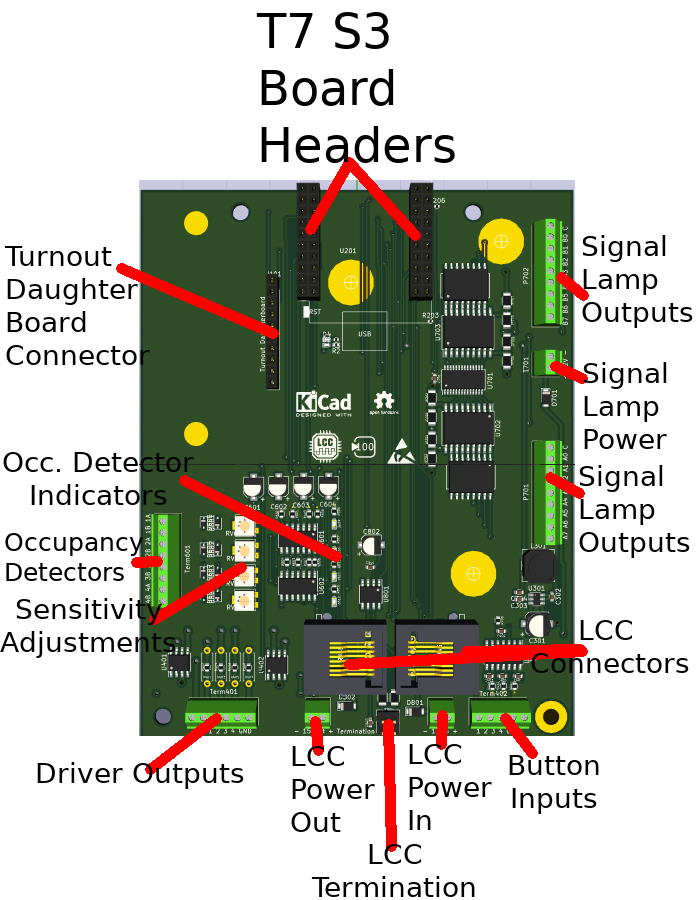
\includegraphics[width=5in]{ESP32-T7S3-MultiFunctionUniversalTurnout-Annotated.png}
\caption{ESP32 T7S3 MultiFunctionUniversalTurnout board, annotated}
\end{centering}\end{figure}

There are various terminal blocks, connectors, and jumper blocks on this
board.  

On the left side is a 10 position socket header for the turnout daughter board
and an 8 position terminal block for the four CT coil occupancy detectors,
Along the bottom is the 6 position terminal block for the driver outputs, then
come the terminal block to extracting power from the LCC bus. Then there is
the termination jumper block for the LCC bus. Then there is terminal block for
injecting power into the LCC bus. Above the LCC power terminal blocks is a
pair of RJ45 connectors. These are for connecting the board to the LCC bus.
These connectors are wired in parallel. On the right side of the board are two
9 position terminal blocks for the signal lamp LEDs. Finally, between the
terminal blocks for the signal lamp LEDs is a two position terminal block to
(optionally) provide power for the signal lamp LEDs.

\subsubsection{Turnout Daughter board connector}

Starting on the upper left, there is a 10 position socket header for the 
turnout daughter board.  The socket mates with the 10 position pin array on 
the underside of the Turnout Daughter board.  The Turnout Daughter boards' 
terminal blocks are described below in Sections~\ref{sect:SM-Daughter}, 
\ref{sect:TS-Daughter}, \ref{sect:SC-Daughter}, and \ref{sect:TC-Daughter}.

\clearpage
\subsubsection{Occupancy Detectors}
\begin{figure}[hbpt]\begin{centering}%
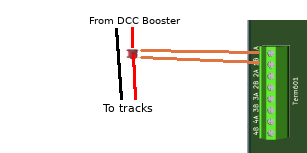
\includegraphics[height=1.5in]{OccupancyDetector-Wiring.png}
\caption{Occupancy Detector Wiring}
\end{centering}\end{figure} 

Then on the lower left side is an 8 position terminal block for the four CT 
coil occupancy detectors.  Each adjacent pair of terminals is for one twisted 
pair cable to one CT coil for one feeder wire for one block. There is a 
sensitivity adjustment trimmer and an indicator LED for each detector.

\subsubsection{Driver Outputs}

There is a 6 position terminal block for the four driver outputs. There are
1500 Ohm load resistors on board, which are suitable for driving LEDs with a
12V supply. There are places for adding through hole load resistors to allow
for increased load current. The driver outputs require an external power
source, typically 12V. The driver chips are totem pole (push-pull), so can
drive both high side and low side, up to 1.5 Amps.

\subsubsection{LCC Power}

Power can be optionally injected into the LCC bus or extracted from the LCC 
bus. Power can be injected to into the LCC bus to power this and other boards. 
Power can also be extracted to power local devices.

\subsubsection{LCC Network Connectors}

There are two RJ45 connectors for the LCC Network. Connect a CAT5 or CAT6
(Ethernet) cable of at least 1 foot in length to the next and previous node in
the network. If this is the last node, only one connector is used and
termination jumpers should be installed. See Section~\ref{sect:termination}.

\subsubsection{Button (or switch) Inputs}

There is a 5 position terminal block for button (or switch) inputs.  These are 
Schmitt-trigger inputs and are referenced to ground (supplied on the fifth 
position of the terminal block).

\subsubsection{PWM Signal Lamp drivers}

There are two 9 position terminal blocks for the sixteen PWM Signal Lamp 
outputs (two banks of 8) and there is a two position terminal blocks to 
provide (optional) external power for the signal lamps.  These terminal blocks 
are on the right side of the board.  The boards can be build to be either for 
common anode or common cathode.

\clearpage
\subsubsection{LCC Termination}
\label{sect:termination}
\begin{figure}[hbpt]\begin{centering}%
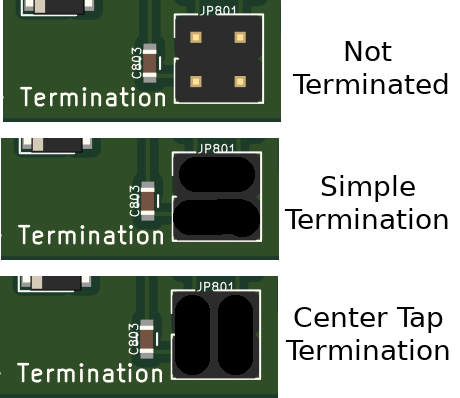
\includegraphics{TerminationJumpers.png}
\caption{Termination Options}
\label{fig:termination}
\end{centering}\end{figure}

There are three options for termination: none, simple, and center tap, as 
shown in Figure~\ref{fig:termination}.


\subsection{Stall Motor Turnout daughter board}
\label{sect:SM-Daughter}
\begin{figure}[hbpt]\begin{centering}%
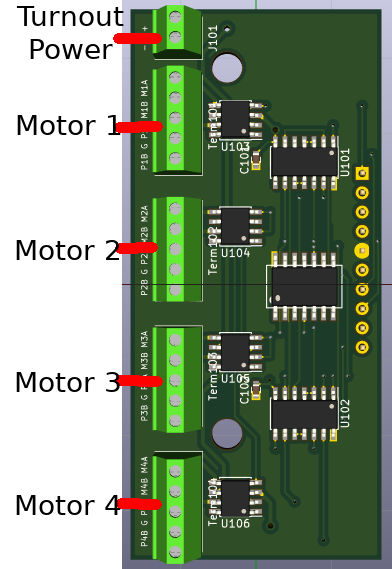
\includegraphics[height=2.5in]{SM-DaughterBoard-Annotated.png}
\caption{Stall Motor Turnout daughter board, annotated}
\end{centering}\end{figure}
\begin{figure}[hbpt]\begin{centering}%
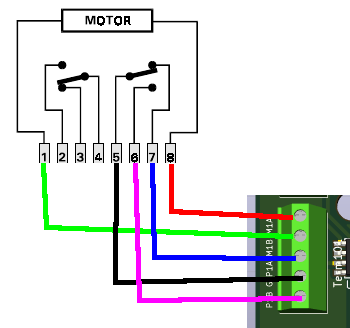
\includegraphics[height=1.5in]{SM-DaughterBoard-TortoiseWiring.png}
\caption{Stall Motor Turnout daughter board, wired to a Tortoise.}
\end{centering}\end{figure}


The Stall Motor Turnout daughter board can drive Circuitron Tortoise and
similar slow motion, stall motor switch machines. There is a 2 position
terminal block for a 12-15 volt supply to drive the stall motors and four 5
position terminal blocks, one for each motor. Each 5 position terminal block
has motor A and B connection for the motors and a point A and B and a ground
(G) connection for the point sense. The motor A and B connections go to the
Tortoises 1 and 8 pins, and the other three can be connected to one of the
poles of the internal switch contacts to report point sense -- the G to the
common.

\subsection{Servo Turnout daughter board}
\label{sect:TS-Daughter}
\begin{figure}[hbpt]\begin{centering}%
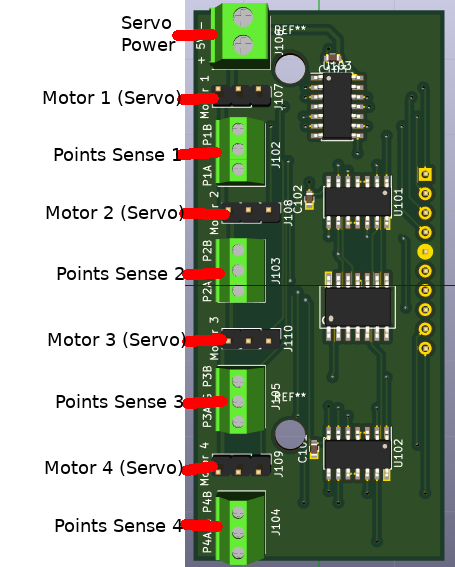
\includegraphics[height=2.5in]{TS-DaughterBoard-Annotated.png}
\caption{Servo Turnout daughter board, annotated}
\end{centering}\end{figure}

The Servo Turnout daughter board can drive standard 5V servos. There a 2
position terminal block for a 5 volt power supply to drive the servos, four
3-pin headers for standard servo connectors, along with four 3 position
terminal blocks for point sense.

\subsection{Single Coil Turnout daughter board}
\label{sect:SC-Daughter}
\begin{figure}[hbpt]\begin{centering}%
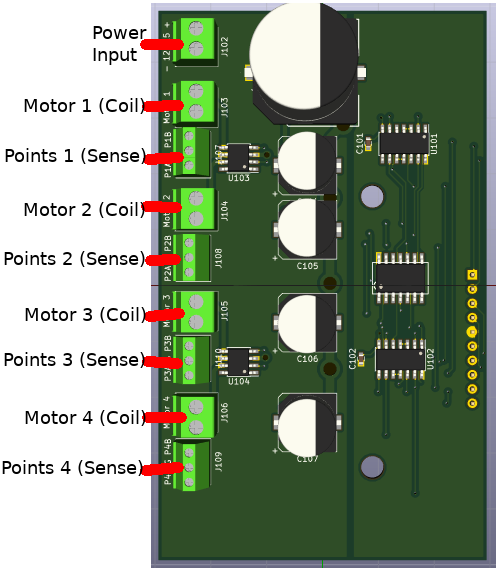
\includegraphics[height=2.5in]{SC-DaughterBoard-Annotated.png}
\caption{Single Coil Turnout daughter board, annotated}
\end{centering}\end{figure}

The Single Coil Turnout daughter board can drive single coil snap action
turnouts, typicaly Kato turnout motors. This a capacitive discharge type
driver circuit. There is a 2 position terminal block for a 12-15 volt power
supply to charge the capacitors.  There is a larger 2 position terminal block 
for each coil, along with a smaller 3 position terminal block point sense for 
each of four turnouts.

\subsection{Twin Coil Turnout daughter board}
\label{sect:TC-Daughter}
\begin{figure}[hbpt]\begin{centering}%
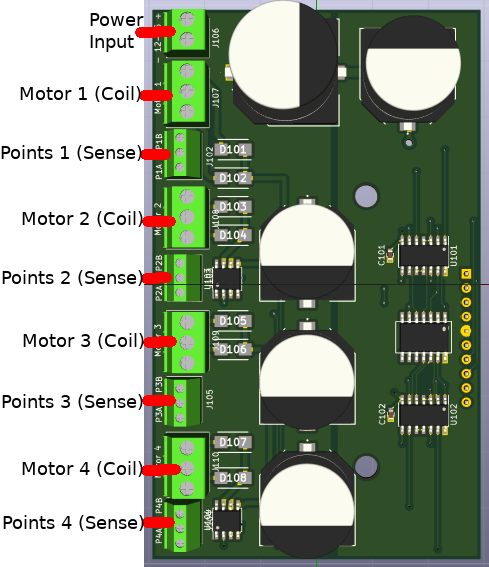
\includegraphics[height=2.5in]{TC-DaughterBoard-Annotated.png}
\caption{Twin Coil Turnout daughter board, annotated}
\end{centering}\end{figure}                                                    
 
The Twin Coil Turnout daughter board can drive twin coil snap action turnouts,
such as Atlas or Peco switch machines. This a capacitive discharge type driver
circuit. There is a 2 position terminal block for a 12-15 volt power supply to
charge the capacitors. There is a larger 3 position terminal block for each
pair of coils, along with a smaller 3 position terminal block point sense for
each of four turnouts.

\clearpage
\section{Application Notes}

In this section I will present four applications:

\begin{enumerate}
\item One end of a siding with local (facia panel) and remote (eg dispatcher
or CTC) control in Section~\ref{sect-appl:siding}.
\item A Yard Throat with track selection in 
Section~\ref{sect-appl:yardthroat}. 
\item A crossing with an interchange track in 
Section~\ref{sect-appl:crossinginterchange}.
\item Automatic Block Signals in Section~\ref{sect-appl:ABS}.
\end{enumerate}

\subsection{Siding with local control panel}
\label{sect-appl:siding}
\begin{figure}[hbpt]\begin{centering}%
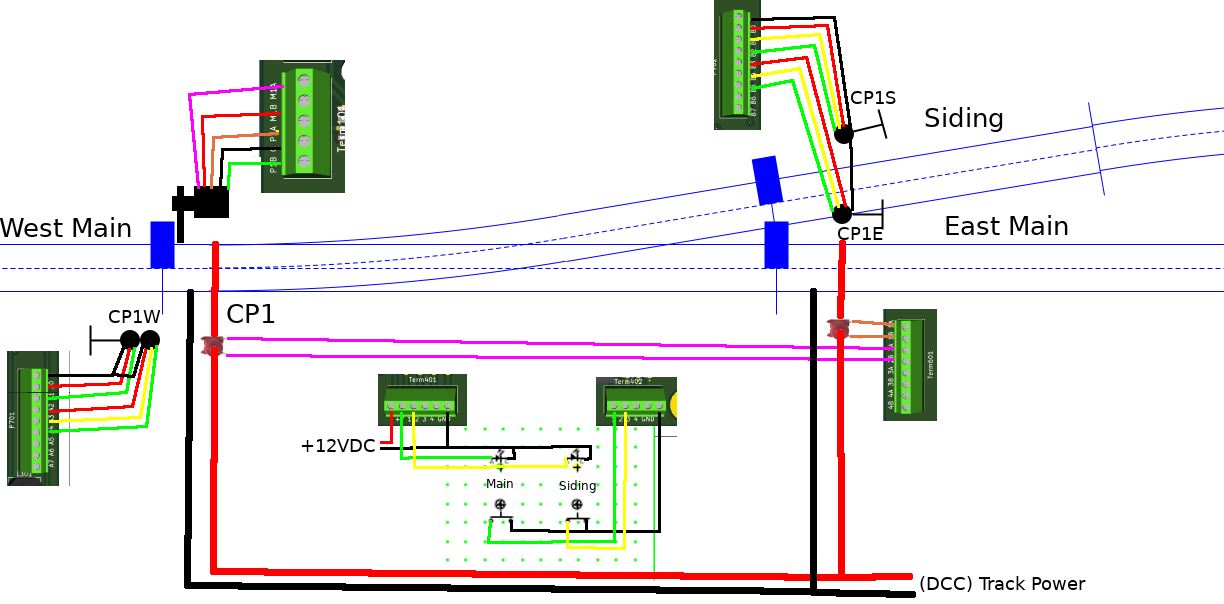
\includegraphics[width=5in]{ExampleSidingCP1-Wiring.png}
\caption{One end of a siding (CP1) with local and remote control, with 
signals.}
\label{fig:ExampleSidingCP1-Wiring}
\end{centering}\end{figure}

This is a basic single turnout with a facia panel with two LEDs indicating the
turnout points' position and two push buttons to select the desired turnout
position. There also is a two headed (3 over 2) interlocking signal at the
turnout's points, and a pair of single head (3 color) signals at the frog
ends. The turnout's wiring is shown in 
Figure~\ref{fig:ExampleSidingCP1-Wiring}. We will use one of the turnout 
drivers (the Stall Motor daughter board is shown, but any of the daughter 
boards could be used), two of the occupancy detectors, two of the LED drivers, 
two of button inputs, and 11 of signal lamp driver outputs.

\begin{figure}[hbpt]\begin{centering}%
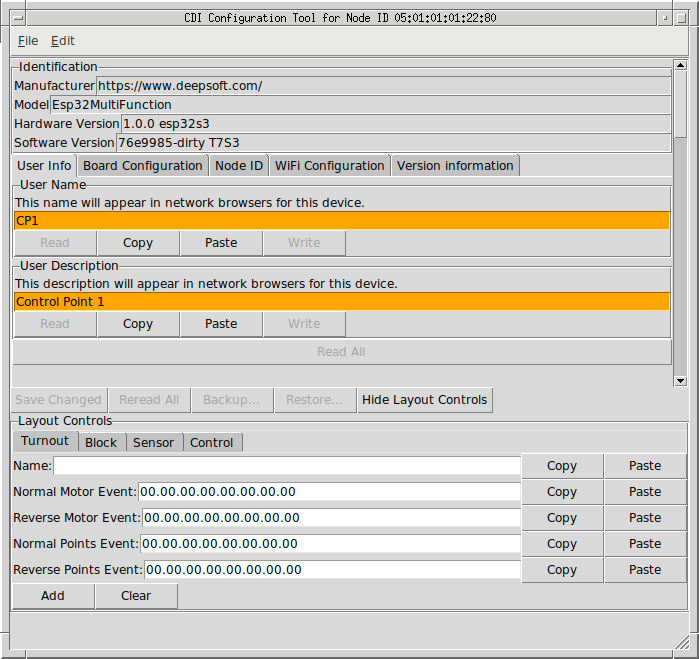
\includegraphics[width=5in]{ExampleSidingCP1-ConfigNameDescr.png}
\caption{Configuring the name and description}
\label{fig:ExampleSidingCP1-ConfigNameDescr}
\end{centering}\end{figure}

We will start by configuring the user name and description of the node, as 
shown in Figure~\ref{fig:ExampleSidingCP1-ConfigNameDescr}.

\begin{figure}[hbpt]\begin{centering}%
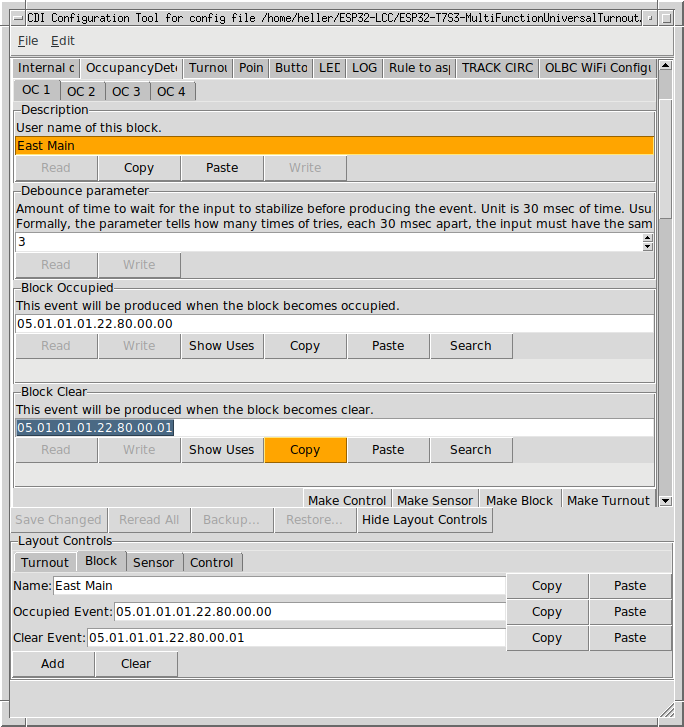
\includegraphics[height=6in]{ExampleSidingCP1-ConfigOC1.png}
\caption{Configuring OC1 and creating Block control item.}
\label{fig:ExampleSidingCP1-ConfigOC1}
\end{centering}\end{figure}
\begin{figure}[hbpt]\begin{centering}%
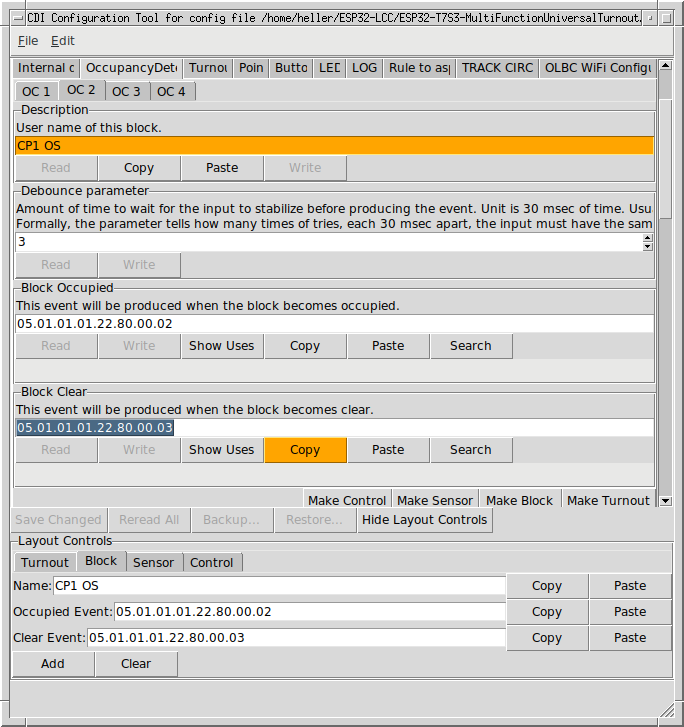
\includegraphics[height=6in]{ExampleSidingCP1-ConfigOC2.png}
\caption{Configuring OC2 and creating Block control item.}
\label{fig:ExampleSidingCP1-ConfigOC2}
\end{centering}\end{figure}

Next, we will move onto the Board Configuration tab and then the Occupancy
Detectors, specificly OC1. Right now, we will just fill in the name (East
Main) and create a Block layout control. Similarly for OC2 (CP1 OS).


\begin{figure}[hbpt]\begin{centering}%
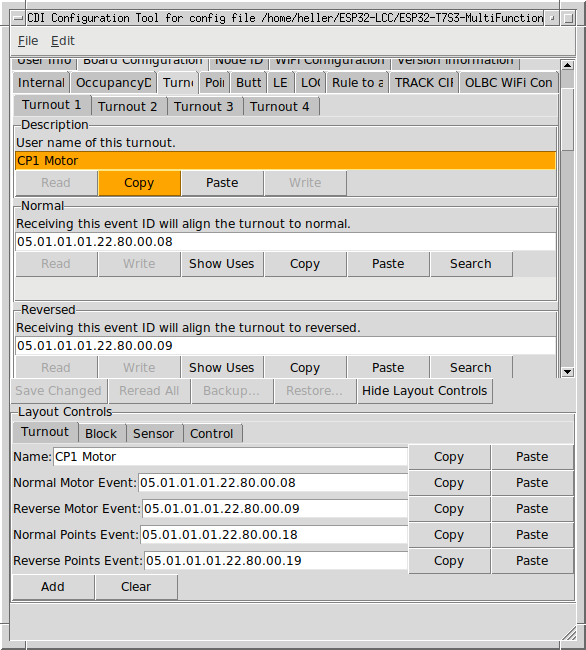
\includegraphics[height=6in]{ExampleSidingCP1-ConfigTurnout1.png}
\caption{Configuring Turnout1 and creating Turnout  control item.}
\label{fig:ExampleSidingCP1-ConfigTurnout1}
\end{centering}\end{figure}
\begin{figure}[hbpt]\begin{centering}%
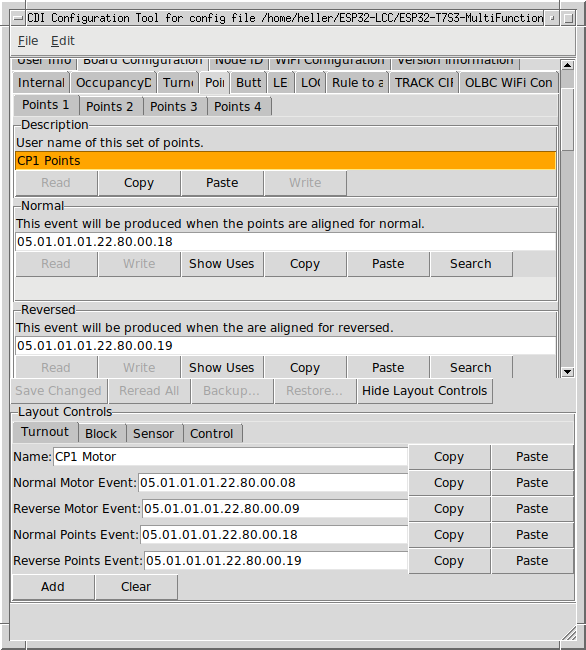
\includegraphics[height=6in]{ExampleSidingCP1-ConfigPoints1.png}
\caption{Configuring Points1 and creating Turnout control item.}
\label{fig:ExampleSidingCP1-ConfigPoints1}
\end{centering}\end{figure}
\begin{figure}[hbpt]\begin{centering}%
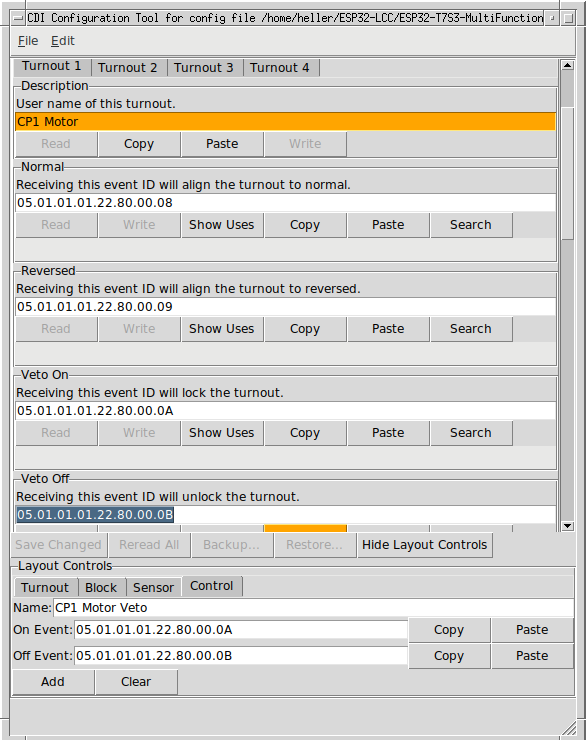
\includegraphics[height=6in]{ExampleSidingCP1-ConfigTurnout-Veto1.png}
\caption{Configuring Turnout Veto control item.}
\label{fig:ExampleSidingCP1-ConfigTurnout-Veto1}
\end{centering}\end{figure}


Similarly we configure the Turnout and Points, along with the veto control
element. Now we set up the logic for the Veto.  We want to enable the turnout 
veto in two cases: dispatcher or OS occupancy, so we need one logic element 
for this.

\begin{figure}[hbpt]\begin{centering}%
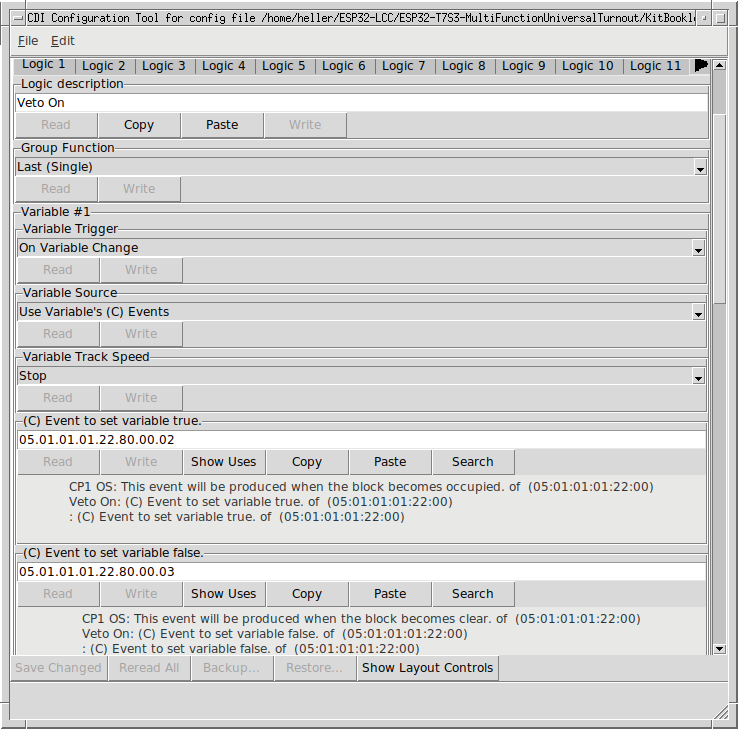
\includegraphics[height=6in]{ExampleSidingCP1-ConfigVetoLogic1a.png}
\caption{Configuring Veto Logic, part1}
\label{fig:ExampleSidingCP1-ConfigVetoLogic1a}
\end{centering}\end{figure}
\begin{figure}[hbpt]\begin{centering}%
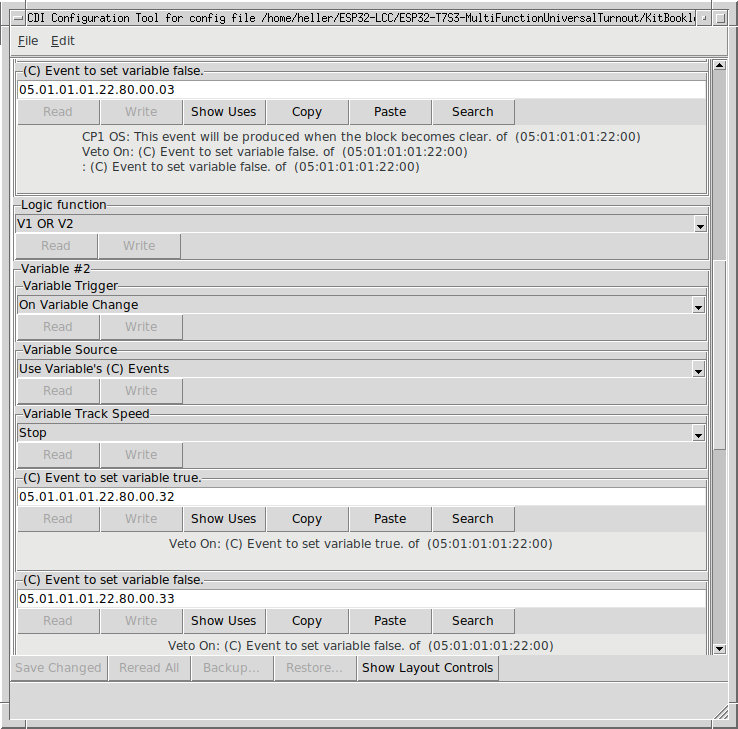
\includegraphics[height=6in]{ExampleSidingCP1-ConfigVetoLogic1b.png}
\caption{Configuring Veto Logic, part2}
\label{fig:ExampleSidingCP1-ConfigVetoLogic1b}
\end{centering}\end{figure}
\begin{figure}[hbpt]\begin{centering}%
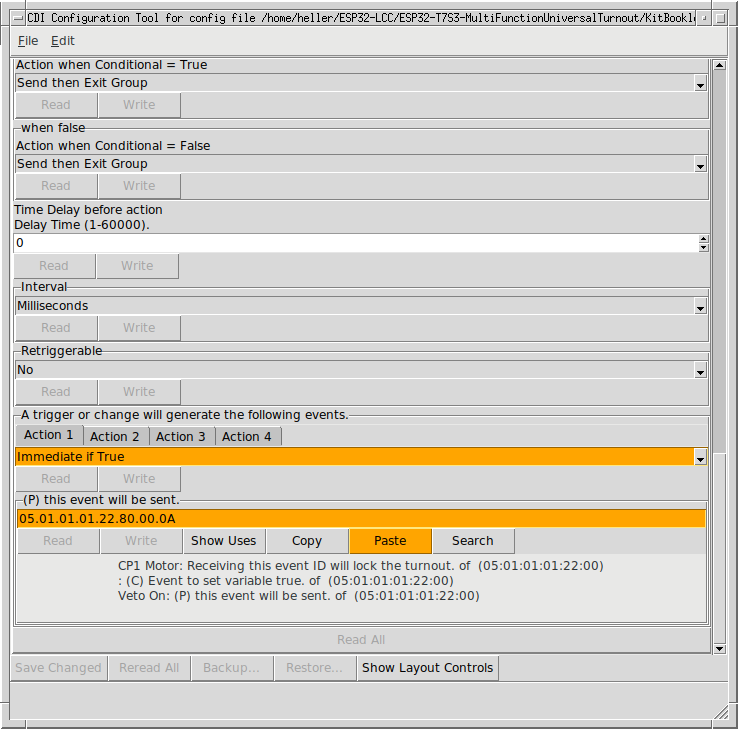
\includegraphics[height=6in]{ExampleSidingCP1-ConfigVetoLogic1c.png}
\caption{Configuring Veto Logic, part3}
\label{fig:ExampleSidingCP1-ConfigVetoLogic1c}
\end{centering}\end{figure}
\begin{figure}[hbpt]\begin{centering}%
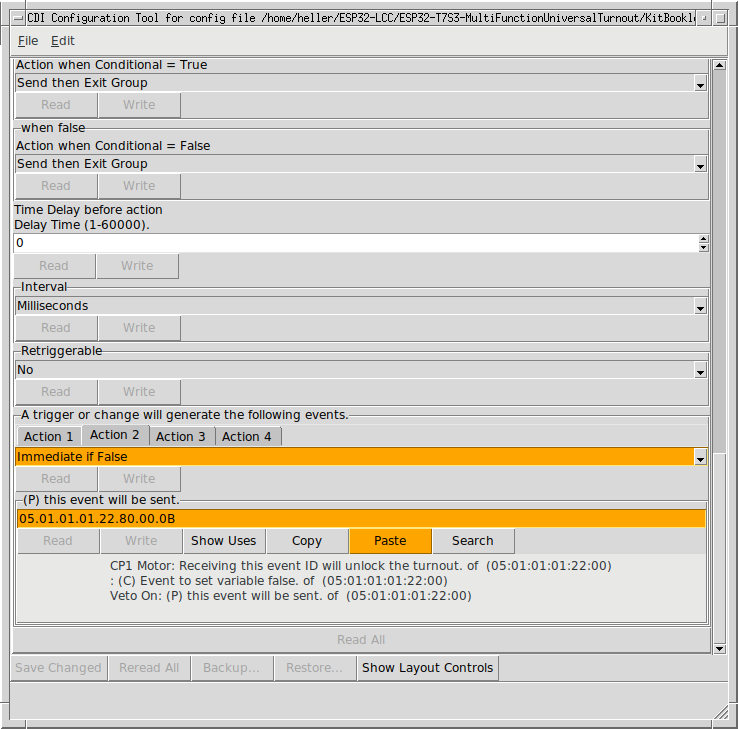
\includegraphics[height=6in]{ExampleSidingCP1-ConfigVetoLogic1d.png}
\caption{Configuring Veto Logic, part 4}
\label{fig:ExampleSidingCP1-ConfigVetoLogic1d}
\end{centering}\end{figure}



\clearpage
\subsection{Yard Throat with track selector}
\label{sect-appl:yardthroat}

\subsection{Crossing with interchange}
\label{sect-appl:crossinginterchange}

\subsection{Automatic Block Signals}
\label{sect-appl:ABS}

\end{document}
